% !TEX root = ../notes_template.tex

\section*{3장 - 연습문제 풀이}

\subsection*{연습문제 \ref{ex-3-1}}

$\gamma_1 = \cos t + i\sin t$, $\gamma_2 = \cos (2t) + i\sin (2t)$,
$\gamma_3 = \cos t - i\sin t$이므로
$k=1,2,3$ 각각의 경우 모두 $(\Re(\gamma_k(t)))^2 + (\Im(\gamma_k(t)))^2=1$이다.
$\gamma_k$의 상은 중심이 $0$이고 반지름이 $1$인 원 $\mathbb T$에 있다.
$\theta \in [0,2\pi)$에 대하여 $z = \exp(i\theta)$이면,
$z = \gamma_1(\theta) = \gamma_2(\theta/2) = \gamma_3(2\pi - \theta)$이다.
따라서 $\mathbb T$위의 모든 점은 $\gamma_1, \gamma_2, \gamma_3$ 각각에 의한 상에
속한다.
\begin{align*}
\int_{\gamma_1} \dfrac1z dz &= \int_0^{2\pi} \dfrac1{\exp(it)}\cdot i\exp(it)dt = 2\pi i, \\
\int_{\gamma_2} \dfrac1z dz &= \int_0^{2\pi} \dfrac1{\exp(2it)}\cdot 2i\exp(2it)dt = 4\pi i, \\
\int_{\gamma_3} \dfrac1z dz &= \int_0^{2\pi} \dfrac1{\exp(-it)}\cdot (-i)\exp(-it)dt = -2\pi i.
\end{align*}

\subsection*{연습문제 \ref{ex-3-2}}

실함수 $x,y$에 대하여 $\gamma(t) = x(t) +iy(t)$, $t\in[0,1]$라 하자.
또한, $u,v$를 각각 함수 $f$의 실수부와 허수부라 하면,
\begin{align*}
f'(\gamma(t))\cdot\gamma'(t)
&= \left( \dfrac{\partial u}{\partial x}(x(t),y(t)) +
i \dfrac{\partial v}{\partial x}(x(t),y(t)) \right) (x'(t) + iy'(t)) \\
&= \dfrac{\partial u}{\partial x}(x(t),y(t)) \cdot x'(t) - \dfrac{\partial v}{\partial x}y'(t) \\
&\qquad +i\left( \dfrac{\partial u}{\partial x}(x(t),y(t)) \cdot y'(t) + \dfrac{\partial v}{\partial x}x'(t) \right) \\
&= \dfrac{\partial u}{\partial x}(x(t),y(t)) \cdot x'(t) + \dfrac{\partial u}{\partial y}y'(t) \\
&\qquad +i\left( \dfrac{\partial v}{\partial y}(x(t),y(t)) \cdot y'(t) + \dfrac{\partial v}{\partial x}x'(t) \right) \\
&\qquad\qquad \text{(코시-리만 방정식을 적용함)} \\
&= \dfrac d{dt} u(x(t), y(t)) + i \dfrac d{dt} v(x(t),y(t)) \quad\text{(연쇄법칙을 적용함)} \\
&= \dfrac d{dt} (u(x(t), y(t)) + i v(x(t),y(t))) = \dfrac d{dt} f(\gamma(t)).
\end{align*}

\subsection*{연습문제 \ref{ex-3-3}}

원형경로 $\gamma$를 $\gamma(t) = 2\exp(it)$, $t\in[0,2\pi]$라 하자.
\begin{itemize}
\item[(1)] 
\begin{align*}
\int_\gamma (z+\bar z) dz & = \int_0^{2\pi} (2\exp(it) + 2\exp(-it))\cdot 2i \cdot \exp(it) dt \\
&= 4i\int_0^{2\pi} (\exp(2it) +1)dt - 4i\cdot 0 + 4i\cdot 2\pi = 8\pi i.
\end{align*}
\item[(2)] 
\begin{align*}
\int_\gamma (z^2-2z+3) dz & = \int_0^{2\pi} (4\exp(2it) - 4\exp(it)+3)\cdot 2i \cdot \exp(it) dt \\
&= \int_0^{2\pi} i(8\exp(3it) - 8\exp(2it) + 6\exp(it))dt  = 0+0+0 =0.
\end{align*}
\item[(3)] 
\begin{align*}
\int_\gamma xy dz & = \int_0^{2\pi}  2\cos t\cdot 2\sin t \cdot 2i \cdot(\cos t +i\sin t) dt \\
&= 4i\int_0^{2\pi} (\sin (2t))(\cos t + i\sin t)dt \\
&= 4i\int_{-\pi}^\pi \underbrace{(\sin(2t))\cos t}_{\text{기함수}} dt
- 2\int_0^{2\pi} (\cos t - \cos(3t))dt \\
&=0 - 2(0-0) = 0.
\end{align*}
\end{itemize}

\subsection*{연습문제 \ref{ex-3-4}}

\begin{itemize}
\item[(1)] $\gamma(t) =(1+i)t$, $t\in[0,1]$이므로,
$\dint_\gamma \Re(z)dz = \dint_0^1 t(1+i)dt = \dfrac{1+i}2$. 
\item[(2)] $\gamma(t) =1+\exp(it)$, $t\in[-\pi/2,0]$이므로, 
\begin{align*}
\int_\gamma \Re(z) dz &= \int_{-\pi/2}^0 (\cos t)i\exp(it)dt
= \int_{-\pi/2}^0 i(\cos t)^2 -(\cos t)(\sin t)dt \\
&= \int_{-\pi/2}^0 \left( i\dfrac{\cos(2t)+1}2 - \dfrac{\sin(2t)}2 \right) dt \\
&= 0 + i\cdot \dfrac12 \cdot \dfrac \pi2 + \dfrac12 = \dfrac12 + i\dfrac\pi4.
\end{align*}
\item[(3)] $\gamma(t) =t+it^ 2$, $t\in[0,1]$이므로,
\[
\int_\gamma \Re(z) dz  = \int_0^1 t\cdot(1+2it)dt = \dfrac12 + 2i\cdot\dfrac13 
=\dfrac12 + \dfrac23i.
\]
\end{itemize}

\subsection*{연습문제 \ref{ex-3-5}}

이항정리에 의하여
\[
(1+z)^n = \sum_{\ell = 0}^n  {n \choose \ell} z^\ell 1^{n-\ell} 
\sum_{\ell = 0}^n  {n \choose \ell} z^\ell.
\]
$0\le k \le n$에 대하여,
\[
\dfrac{(1+z)^n}{z^{k+1}} =\sum_{\ell = 0}^n  {n \choose \ell} z^{\ell-k-1}
\]
이므로
\begin{align*}
\dfrac1{2\pi i} \int_C \dfrac{(1+z)^n}{z^{k+1}}dz
&= \dfrac1{2\pi i} \int_C \sum_{\ell = 0}^n  {n \choose \ell} z^{\ell-k-1} dz \\
&  \sum_{\ell = 0}^n  {n \choose \ell} \dfrac1{2\pi i} \int_C  z^{\ell-k-1}dz
= {n \choose k}.
\end{align*}

\subsection*{연습문제 \ref{ex-3-6}}
\begin{itemize}
\item[(1)]
$U_f, V_f, U_g, V_g:[a,b] \to \mathbb R$에 대하여
$f(\gamma(t))\gamma'(t) = U_f(t) + iV_f(t)$,
$g(\gamma(t))\gamma'(t) = U_g(t) + iV_g(t)$, $t\in[a,b]$라고 하자.

\begin{align*}
\int_\gamma (f+g)(z)dz
&= \int_a^b (f+g)(\gamma(t))\cdot \gamma'(t)dt \\
&= \int_a^b \left( f(\gamma(t))\cdot \gamma'(t) + g(\gamma(t))\cdot \gamma'(t) \right) dt\\
&= \int_a^b (U_f(t) + U_g(t)) dt + i \int_a^b (V_f(t) + V_g(t)) dt \\
&= \int_a^b U_f(t)dt + \int_a^b V_f(t)dt + i\int_a^b V_f(t)dt + i\int_a^b V_g(t)dt \\
&= \int_\gamma f(z)dz + \int_\gamma g(z)dz.
\end{align*}

\item[(2)] $\alpha = p+iq$ ($p,q\in\mathbb R$)이고
$U,V:  [a,b] \to \mathbb R$에 대하여
$f(\gamma(t))\gamma'(t)  = U(t) + iV(t)$, $t\in[a,b]$라 하자.
그러면,
\begin{align*}
\int_\gamma (\alpha\cdot f)(z) dz
&= \int_a^b (p+iq)(U(t) + iV(t))dt \\
&= \int_a^b(pU(t) - qV(t))dt + i\int_a^b (pV(t) + qU(t))dt \\
&= p \left(\int_a^b U(t)dt + i \int_a^b V(t)dt \right)
+ iq\left(\int_a^b U(t)dt + i \int_a^b V(t)dt \right) \\
&= (p+iq)\left(\int_a^b U(t)dt + i \int_a^b V(t)dt \right)
= \alpha \cdot \int_\gamma f(z)dz.
\end{align*}
\end{itemize}

\subsection*{연습문제 \ref{ex-3-7}}

$-(-\gamma): [a,b] \to \mathbb C$는 다음 식으로 주어진다.
\[
(-(-\gamma))(t)= (-\gamma)(a+b-t) = \gamma(a+b-(a+b-t)) = \gamma(t),
\quad t\in[a,b].
\]
따라서 $-(-\gamma) = \gamma$이며, 그림으로 보면 직관적으로 명백하다.

\subsection*{연습문제 \ref{ex-3-8}}

$\gamma(b) = (-\gamma)(a)$이므로
$\gamma$와 $-\gamma$는 결합가능한 경로이다.
\[
\int_{\gamma+(-\gamma)} f(z) dz = \int_\gamma f(z) dz + \int_{-\gamma} f(z)dz
=  \int_\gamma f(z) dz - \int_\gamma f(z) dz = 0.
\]

\subsection*{연습문제 \ref{ex-3-9}}

$\gamma:[0,1] \to \mathbb C$를 $\gamma(t) = (1+i)t$, $t\in [0,1]$이라 하자.
피타고라스 정리를 쓰면, $\gamma$의 길이는 $\sqrt{1^2+1^2} = \sqrt{2}$.

\begin{figure*}[h!]
\begin{center}
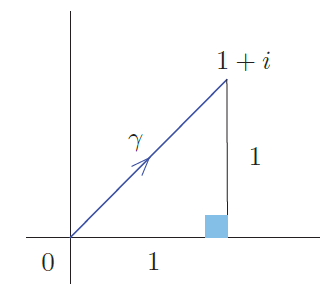
\includegraphics[width=0.3\textwidth]{./Solution/figs/fig-s-0-8}
\end{center}
%\caption{$\left\{ z \in\mathbb C \,:\, z\ne0, \dfrac\pi4 < |\Arg(z)| < \dfrac\pi3 \right\}$}
%\label{fig-5-14}
\end{figure*}

또한 $|(\gamma(t))^2| = |t+it|^2 = 2t^2$이고,
$\max\limits_{t\in[0,1]} |(\gamma(t))^2| = 2\cdot 1^2 = 2$.
따라서
\[
\left| \int_\gamma z^2dz \right|
\le \left( \max\limits_{t\in[0,1]} |(\gamma(t))^2|  \right) \cdot
(\text{$\gamma$의 길이})
= 2\sqrt{2}.
\]
직접 계산하면,
\begin{align*}
\int_\gamma z^2 dz = \int_0^1 (t+it)^2\cdot(1+i)dt
= \int_0^1 (1+i)^3t^2dt = \dfrac{(1+i)^3}3
\end{align*}
이므로
$\left| \dint_\gamma z^2 dz \right| = \dfrac{(\sqrt{3})^3}3 = \dfrac{2\sqrt{2}}3$.

\subsection*{연습문제 \ref{ex-3-10}}

\begin{align*}
{2n \choose n} = \left|  {2n \choose n} \right|
&= \left| \dfrac1{2\pi i}\int_C \dfrac{(1+z)^{2n}}{z^{n+1}}dz \right| \\
&\le \dfrac1{2\pi} \left( \max_{|z|=1} \left| \dfrac{(1+z)^{2n}}{z^{n+1}}\right| \right)
\cdot 2\pi\cdot 1 = \max_{|z|=1} \dfrac{|1+z|^{2n}}1 \\
&\le (1+1)^{2n} = 2^{2n} = 4^n.
\end{align*}

\subsection*{연습문제 \ref{ex-3-11}}

$F=U+iV$를 $\bar z \in \mathbb C$의 부정적분이라고 하자.
그러면,
\[
\dfrac{\partial U}{\partial x}  + i \dfrac{\partial V}{\partial x}
= \dfrac{\partial V}{\partial y} - i\dfrac{\partial U}{\partial y}
= F' = \bar z = x-iy.
\]

$x_0\in\mathbb R$을 고정하자. 그러면 $(x,y)\in\mathbb R^2$에 대하여
\[
V(x,y ) - V(x_0, y) = \int_{x_0}^x \dfrac{\partial V}{\partial x}(\xi, y )d\xi
= \int_{x_0}^x -y d\xi = -xy +x_0y.
\]
따라서 $V(x,y) = -xy + \varphi(y)$, $\varphi(y):+V(x_0,y_0) + x_0y$이면,
\[
x  = \dfrac{\partial V}{\partial y} = -x + \varphi'(y).
\]
즉, 모든 $x\in\mathbb R$에 대하여 $\varphi'(y) = 2x$인데
이는 분명 모순이다.
특히, $2\cdot 1 = 2 = \varphi'(y) = 2\cdot  0 = 0$.

\subsection*{연습문제 \ref{ex-3-12}}

$(fg)' = fg' + f'g$이므로
함수 $\zeta \mapsto f(\zeta)g'(\zeta) + f'(\zeta)g(\zeta)$는 
부정적분을 갖는다.
따라서 경로적분의 기본정리에 의하여
\[
\int_\gamma \left( f(\zeta)g'(\zeta) + f'(\zeta)g(\zeta) \right) d\zeta
= f(z)g(z) - f(w)g(w)
\]
이고 이를 정리하면 원하는 결과를 얻는다.

\subsection*{연습문제 \ref{ex-3-13}}

$\mathbb C$에서 $\sin' z = \cos z$이므로 $\cos z$는 부정적분을 갖는다.
따라서 경로적분의 기본정리에 의하여
\begin{align*}
\int_\gamma \cos z \, dz 
&= \sin i - \sin (-i) = 2\sin i = 2\dfrac{\exp(i\cdot i) - \exp(-i\cdot i)}{2i}
= \dfrac{e^{-1} - e^{1}}i \\
&= \left( e - \dfrac1e \right)i.
\end{align*}


\subsection*{연습문제 \ref{ex-3-14}}

$\mathbb C$에서  $\exp' z = \exp z$이므로
$0$과 $a+ib$를 잇는 경로 $\gamma$를 따라 적분하면
\[
\int_\gamma \exp z\, dz = \exp(a+ib) - \exp 0 = e^a(\cos b + i \sin b) -1
= e^a\cos b -1 +ie^a\sin b.
\]
 경로를 $\gamma(x) = (a+ib)x$, $x\in[0,1]$로 잡으면,
\[
\int_\gamma \exp z\, dz = \int_0^1 \exp(a+ib)\cdot (a+ib)dx
= \int_0^1 e^{ax}(\cos(bx) + i\sin(bx))(a+ib)dx.
\]
 따라서,
$(a-ib)\dint_\gamma \exp z\, dz = \dint_0^1 e^{ax}(\cos(bx) + i\sin(bx))(a^2+b^2)dx$이고,
\begin{align*}
(a^2+b^2) \int_0^1 e^{ax} \cos (bx)dx
&= \Re\left( (a-ib)\int_\gamma \exp z\, dz \right) \\
&= \Re((a-ib)(e^a\cos b -1 + ie^a\sin b)) \\
&= a(e^a\cos b -1) + be^a \sin b.
\end{align*}
즉,
$\dint_0^1 e^{ax}\cos(bx)\, dx = \dfrac{a(e^a\cos b - 1) + be^a\sin b}{a^2+b^2}$.

\subsection*{연습문제 \ref{ex-3-15}}

중심이 $0$이고 반지름 $r>0$인 원을 반시계방향으로 도는 닫힌경로 $C$를 생각하자.
$C(\theta) = r\exp(i\theta)$, $\theta\in[0,2\pi]$.
경로적분의 기본정레에 의해
\begin{align*}
0 & = \int_C \exp z \, dz = \int_0^{2\pi} e^{r\cos\theta +ir\sin\theta}
\cdot ri\exp(i\theta)d\theta\\
&= \int_0^{2\pi} e^{r\cos\theta} \cdot r\cdot i \exp(i(r\sin\theta +\theta))d\theta.
\end{align*}
위 식에서 실수부만 취하면
\[
\int_0^{2\pi} e^{r\cos\theta} \cos(r\sin \theta + \theta)d\theta = 0.
\]

\subsection*{연습문제 \ref{ex-3-16}}

$\mathbb C\setminus\{0\}$에서 복소미분가능한 $F$가 $F'=1/z$를 만족한다고 하자.
중심이 $0$이고 반시계방향으로 도는 원형경로 $C$를 생각하자.
$C$가 닫힌경로 이므로, 경로적분의 기본정리에 의해
\[
\int_C F'(z)dz = 0.
\]
한편, 이미 알고있는 계산 결과에 따르면,
\[
\int_C F'(z)dz = \int_C \dfrac1z dz = 2\pi i
\]
이므로 모순이다.

\subsection*{연습문제 \ref{ex-3-17}}

(ER1)
$\gamma: [0,1] \to D$가 닫힌경로라고 하자.
$H:[0,1]\times[0,1] \to D$를 $H(t,s) = \gamma(t)$, $t,s\in[0,1]$로 정의하면,
$H$는 연속이고,
\begin{align*}
H(t,0) &=\gamma(t), \quad t\in[0,1],\\
H(t,1) &=\gamma(t), \quad t\in[0,1],\\
H(0,s) &=\gamma(0) = \gamma(1) = H(1,s), \quad s\in[0,1].
\end{align*}
따라서 $\gamma$는 자기자신과 $D$-호모토픽하다.
즉, 관계는 반사적(reflexive)이다.
(ER2)
$\gamma_0, \gamma_1: [0,1] \to D$가 닫힌경로이고
$\gamma_0$가 $\gamma_1$과 $D$-호모토픽하다고 하자.
그러면, 다음을 만족하는 연속함수 $H:[0,1]\times[0,1] \to D$가 존재한다.
\begin{align*}
H(t,0) &= \gamma_0(t), \quad t\in [0,1], \\
H(t,1) &= \gamma_1(t), \quad t\in [0,1], \\
H(0,s) &= H(1,s), \quad s\in [0,1].
\end{align*}
$\tilde H:[0,1]\times [0,1] \to D$를
$\tilde H(t,s) = H(t,-s)$, $t,s\in[0,1]$로 정의하자.
그러면, $\tilde H$는 연속이고 다음을 만족한다.
\begin{align*}
\tilde H(t,0) & = H(t,1) = \gamma_1(t), \quad t\in[0,1], \\
\tilde H(t,1) & = H(t,0) = \gamma_0(t), \quad t\in[0,1], \\
\tilde H(0,s) & = H(0,1-s) = H(1,1-s) = \tilde H(1,s), \quad s\in[0,1].
\end{align*}
따라서 $\gamma_1$은 $\gamma_0$와 $D$-호모토픽하다.
즉, 관계는 대칭적(symmetric)이다.

(ER3)
$\gamma_0, \gamma_1, \gamma_2$가 닫힌경로이고
$\gamma_0$가 $\gamma_1$과 $D$-호모토픽하고,
$\gamma_1$이 $\gamma_2$와 $D$-호모토픽하다고 하자.
그러면, 다음을 만족하는 연속함수  $H, K:[0,1]\times[0,1]\to D$가 존재한다.
\begin{align*}
H(t,0) = \gamma_0(t), \ t\in[0,1], \quad & K(t,0) = \gamma_1(t), \ t\in[0,1], \\
H(t,1) = \gamma_1(t), \ t\in[0,1], \quad & K(t,1) = \gamma_2(t), \ t\in[0,1], \\
H(0,s) = H(1,s), \ s\in[0,1], \quad & K(0,s) = K(1,s), \ s\in[0,1].
\end{align*}
$L:[0,1]\times[0,1]\to D$를
\[
L(t,s) = \begin{cases}
H(t,2s), & s\in [0, \frac12], \\
K\left(t, 2(s-\frac12)\right), & s\in (\frac12,1]
\end{cases}
\]
로 정의하면,
\begin{align*}
L(t,0) &= H(t,0) = \gamma_0(t), \quad t\in[0,1],\\
L(t,1) &= K(t,1) = \gamma_2(t), \quad t\in[0,1].
\end{align*}
또한, $0\le s\le \frac12$에 대하여 $L(0,s) = H(0,2s) = H(1,2s) = L(1,s)$, 
$\frac12 <s\le1$에 대하여
\[
L(0,s) = K\left( 0, 2(s - \frac12) \right) = K\left( 1, 2(s - \frac12) \right) = L(1,s).
\]
이다.

$[0,1]\times (\frac12,1]$에서 정의된 수열 $((t_n, s_n))_{n\in\mathbb N}$이
$(t_0,\frac12)$에 수렴한다면,
\begin{align*}
\lim_{n\to\infty} L(t_n, s_n)
& = \lim_{n\to\infty} K\left( t_n, 2(s_n - \frac12)\right)
= K(t_0,0) = \gamma_1(t_0) \\
&= H(t_0,1) = L\left( t_0, \frac12\right) = L\left( \lim_{n\to\infty} (t_n, s_n) \right).
\end{align*}
따라서 $L$은 연속함수이다.
결론적으로, $\gamma_0$는 $\gamma_2$와 $D$-호모토픽하다.
즉, 관계는 추이적(transitive)이다.

이상에서 $D$-호모토피 관계는 반사적, 대칭적, 추이적인 성질을 만족하므로
동치(equivalence) 관계이다.

\subsection*{연습문제 \ref{ex-3-18}}

그림에서 경로 $C$는 경로 $S$와 $\mathbb C\setminus \{0\}$-호모토픽함을 알 수 있다.

\begin{figure*}[h!]
\begin{center}
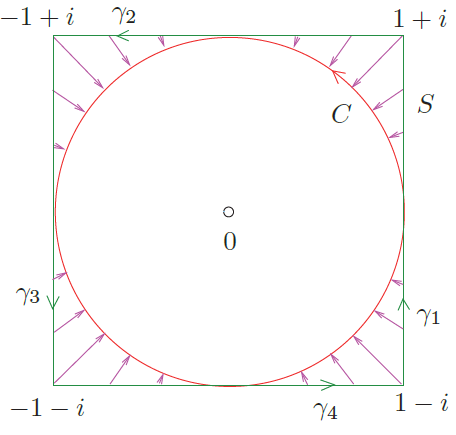
\includegraphics[width=0.4\textwidth]{./Solution/figs/fig-s-0-9}
\end{center}
%\caption{$\left\{ z \in\mathbb C \,:\, z\ne0, \dfrac\pi4 < |\Arg(z)| < \dfrac\pi3 \right\}$}
%\label{fig-5-14}
\end{figure*}

직접 계산을 위해 $t\in[0,1]$에 대하여 경로를 다음과 같이 정의하자.
\begin{align*}
\gamma_1(t) &:= (1-t)(1-i) + t(1+i) = 1 + i(2t-1), \\
\gamma_2(t) &:= (1-t)(1+i) + t(-1+i) = (1-2t) + i, \\
\gamma_3(t) &:= (1-t)(-1+i) + t(-1-i) = -1 + i(1-2t), \\
\gamma_4(t) &:= (1-t)(-1-i) + t(1-i) = 2t-1 -i.
\end{align*}
그러면,
\[
\int_S \dfrac1z dz = \int_{\gamma_1} \dfrac1z dz
+ \int_{\gamma_2} \dfrac1z dz + \int_{\gamma_3} \dfrac1z dz + \int_{\gamma_4} \dfrac1z dz
\]
이므로,
\begin{align*}
\int_{\gamma_1} \dfrac1z dz
&= \int_0^1 \dfrac{2i}{1+i(2t-1)}dt = \int_0^1 \dfrac{2i(1-i(2t-1))}{1+(2t-1)^2}dt \\
&= 2i\int_0^1\dfrac1{1+(2t-1)^2}dt + 2\int_0^1 \dfrac{2t-1}{1+(2t-1)^2}dt \\
&\stackrel{(u=2t-1)}{=} i \int_{-1}^1 \dfrac1{1+u^2}du  + \int_{-1}^1 \dfrac u{1+u^2}du \\
&= i(\tan^{-1}1 - \tan^{-1}(-1)) + 0 
= i\left(\dfrac\pi4 - \left(-\dfrac\pi4\right)\right) = i \dfrac\pi2.
\end{align*}
같은 방법으로, 
\[
\int_0^1 \dfrac2{1+(2t-1)^2}dt = \dfrac\pi2, \quad
\int_0^1 \dfrac{2t-1}{1+(2t-1)^2}dt = 0,
\]
을 이용하면,
\begin{align*}
\int_{\gamma_2} \dfrac1z dz
&= \int_0^1 \dfrac{-2}{1-2t+i}dt = \int_0^1 \dfrac{-2\cdot(-(2t-1)-i)}{1+(2t-1)^2}dt \\
&= 0 + (-1)(-i)\dfrac\pi2 = i\dfrac\pi2, \\
\int_{\gamma_3} \dfrac1z dz
&= \int_0^1 \dfrac{-2i}{-1+i(1-2t)}dt = \int_0^1 \dfrac{-2i\cdot(-1+i(2t-1))}{1+(2t-1)^2}dt \\
&= -i\cdot(-1)\cdot\dfrac\pi2 +0 = i\dfrac\pi2, \\
\int_{\gamma_4} \dfrac1z dz
&= \int_0^1 \dfrac{2}{2t-1-i}dt = \int_0^1 \dfrac{2\cdot((2t-1)+i)}{1+(2t-1)^2}dt \\
&= 0 + i\dfrac\pi2 +0 = i\dfrac\pi2.
\end{align*}
따라서 예상대로 $\dint_S \dfrac1z dz = 4\cdot\left(i\dfrac\pi2\right) = 2\pi i$가 된다.

\subsection*{연습문제 \ref{ex-3-19}}

중심이 $0$이고 반시계방향으로 도는 원형경로 $C$에 대하여
\[
\int_C \dfrac 1z dz = 2\pi i.
\]
한편 그림 \ref{fig-5-17}\과 같이 타원형 경로 $E$는 $C$와 
$\mathbb C\setminus \{0\}$-호모토픽하다.

\begin{figure}[h!]
\begin{center}
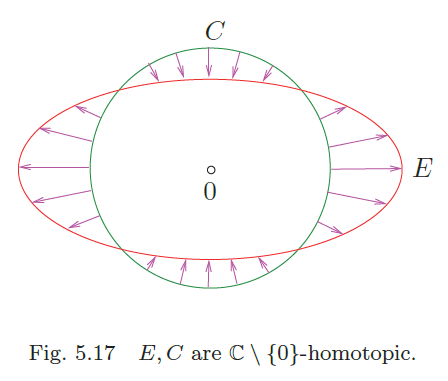
\includegraphics[width=0.4\textwidth]{./Solution/figs/fig-5-17}
\end{center}
\caption{$\mathbb C\setminus \{0\}$-호모토픽한 경로 $E$와 $C$}
\label{fig-5-17}
\end{figure}

따라서 코시 적분정리에 의해 $\dint_E \dfrac 1z dz = \dint_C \dfrac1z dz = 2\pi i$이고,
\begin{align*}
2\pi i &= \int_E \dfrac 1z dz = \int_0^{2\pi} \dfrac1{a\cos\theta +i b\sin\theta}
\cdot(-a\sin\theta + ib\cos\theta)d\theta \\
&= \int_0^{2\pi} \dfrac{(-a\sin\theta +ib\cos\theta)(a\cos\theta -ib\sin\theta)}
{a^2(\cos\theta)^2 + b^2(\sin\theta)^2}d\theta \\
&= \int_0^{2\pi} \dfrac{(b^2-a^2)(\cos\theta)(\sin\theta)+iab((\cos\theta)^2+(\sin\theta)^2)}
{a^2(\cos\theta)^2 + b^2(\sin\theta)^2}d\theta \\
&= \int_0^{2\pi} \dfrac{(b^2-a^2)(\cos\theta)(\sin\theta)+iab\cdot 1}
{a^2(\cos\theta)^2 + b^2(\sin\theta)^2}d\theta.
\end{align*}
허수부를 비교하면,
$\dint_0^{2\pi} \dfrac1{a^2(\cos\theta)^2 + b^2(\sin\theta)^2}d\theta = \dfrac{2\pi}{ab}$.

\subsection*{연습문제 \ref{ex-3-20}}

\begin{figure}[h!]
\begin{center}
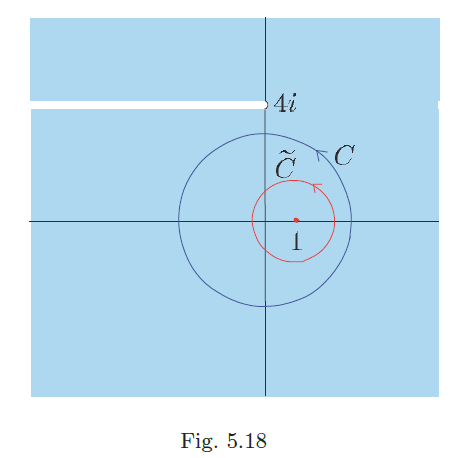
\includegraphics[width=0.4\textwidth]{./Solution/figs/fig-5-18}
\end{center}
\caption{적분경로 $C$, $\tilde C$}
\label{fig-5-18}
\end{figure}

그림 \ref{fig-5-18}을 참고하라.

\begin{itemize}
\item[(1)]  $z\mapsto \Log(z-4i)$는 $\mathbb C \setminus \{r+4i \,:\, r\le0\}$에서
복소해석함수이다. 따라서 코시 적분정리를 쓰면,
\[
\int_C \Log (z-4i)dz = 0.
\]
\item[(2)] $\tilde C$가 중심이 $1$이고 반지름 $r>0$인 원이라 하면,
\[
\int_{\tilde C} \dfrac1{z-1} dz = 2\pi i
\]
임을 알고 있다.
$1/(\cdot -1)$이 $\mathbb C\setminus\{1\}$에서 복소해석함수이고
원형경로 $C$와 $\tilde C$는 $\mathbb C\setminus\{1\}$-호모토픽이므로,
코시 적분정리에 의해,
\[
\int_C \dfrac1{z-1} dz = \int_{\tilde C} \dfrac1{z-1}dz = 2\pi i.
\]
\item[(3)] 
\begin{align*}
i^{z-3} &= \exp((z-3)\Log i) = \exp\left( (z-3)\left( \log 1 + i\dfrac\pi2\right)\right) \\
&= \exp\left( (z-3)\left(0+i\dfrac\pi2\right)\right) \\
&= \exp\left( i\dfrac\pi2 \cdot(z-3)\right).
\end{align*}
따라서 $z\mapsto i^{z-3}$은 전해석함수이다.
코시 적분정리에 의해
\[
\int_C i^{z-3}dz = 0.
\]
\end{itemize}

\subsection*{연습문제 \ref{ex-3-21}}

\begin{itemize}
\item[(1)] 
\[
\varphi'(t) = \exp\left( \int_0^t \dfrac{\gamma'(s)}{\gamma(s)}ds \right)
\cdot \dfrac d{dt}\left( \int_0^t \dfrac{\gamma'(s)}{\gamma(s)}ds \right) 
= \varphi(t)\cdot \dfrac{\gamma'(t)}{\gamma(t)}
\]
에서 $\varphi'\gamma - \varphi\gamma' = 0$이고,
\[
\dfrac d{dt} \left( \dfrac\varphi \gamma \right) 
= \dfrac{\varphi'\gamma - \varphi\gamma'}{\gamma^2} = \dfrac0{\gamma^2} = 0.
\]
따라서 $\dfrac{\varphi(0)}{\gamma(0)}=\dfrac{\varphi(1)}{\gamma(1)}$.
그런데, $\gamma$가 닫힌경로이므로 $\gamma(0)=\gamma(1)$이므로,
\[
\varphi(1) = \varphi(0) = \exp\left( \int_0^0 \dfrac{\gamma'(s)}{\gamma(s)}ds \right)
= \exp(0) = 1.
\]
결론적으로, $w(\gamma) \in\mathbb Z$.
\item[(2)] $\Gamma_1(t) = \exp(2\pi i t)$ ($t\in[0,1]$)의 회전수는
\begin{align*}
w(\Gamma_1) &= \dfrac1{2\pi i} \int_0^1 \dfrac{\Gamma_1'(t)}{\Gamma_1(t)} dt \\
&=\dfrac1{2\pi i} \int_0^1 \dfrac{2\pi i\exp(2\pi i t)}{\exp(2\pi i t)}dt \\
&=\dfrac1{2\pi i} \cdot 2\pi i  = 1.
\end{align*}
\item[(3)]  $(\gamma_1\cdot\gamma_2)'(t) = \gamma_1'(t)\gamma_2(t) +
\gamma_1(t)\gamma_2'(t)$, $t\in[0,1]$이므로,
\begin{align*}
w(\gamma_1\cdot\gamma_2)
&= \dfrac1{2\pi i} 
\int_0^1 \dfrac{(\gamma_1\cdot\gamma_2)'(t)}{(\gamma_1\cdot\gamma_2)(t)}dt\\
&= \dfrac1{2\pi i} \int_0^1 \dfrac{\gamma_1'(t)\gamma_2(t) +\gamma_1(t)\gamma_2'(t)}
{(\gamma_1\cdot\gamma_2)(t)}dt \\
&= \dfrac1{2\pi i} \int_0^1 \dfrac{\gamma_1'(t) \cancel{\gamma_2(t)}}
{\gamma_1(t) \cancel{\gamma_2(t)}}dt 
+ \dfrac1{2\pi i} \int_0^1 \dfrac{\cancel{\gamma_1(t)}\gamma_2'(t)}
{\cancel{\gamma_1(t)}\gamma_2(t)}dt  \\
&= w(\gamma_1) + w(\gamma_2).
\end{align*}
\item[(4)] $\Gamma_m = \Gamma_1 \cdot\cdots\cdot \Gamma_1$ ($m$번 곱)이므로
\begin{align*}
w(\Gamma_m) &= w(\Gamma_1) + \cdots + w(\Gamma_1) \ \ (m\text{번}) \\
&= m\cdot w(\Gamma_1) = m\cdot 1 = m.
\end{align*}
\item[(5)] 함수 $\varphi:[0,1]\to \mathbb R$를 
원점에서 $\gamma_0(t)$까지의 거리 $\varphi(t) = |\gamma_0(t)|$, $t\in[0,1]$로 정의하자.
$\gamma_0$가 $0$을 지나지 않고, $\varphi$는 연속함수이기 때문에
최솟값 $d_0$ ($d_0>0$)를 갖는다.
$\delta = d_0/2 >0$로 택하자.
$\gamma$가 
\[
\|\gamma - \gamma_0\| := \max_{t\in[0,1]} | \gamma(t) - \gamma_0(t)| < \delta
\]
를 만족하는 매끄러운 닫힌경로라고 하자.
그러면
$\gamma$가 $\gamma_0$와 $\mathbb C\setminus \{0\}$-호모토픽함을 증명하고자 한다.
$H:[0,1]\times[0,1]\to \mathbb C\setminus\{0\}$를 
$H(t,s) = (1-s)\gamma_0(t) + s\gamma(t)$, $t,s\in[0,1]$로 정의하면
$H$는 연속함수이고,
\begin{align*}
H(t,0) &= \gamma_0(t), \quad t\in[0,1],\\
H(t,1) &= \gamma(t), \quad t\in[0,1],\\
H(0,s) &= (1-s)\gamma_0(0) + s\gamma(0) \\
&= (1-s)\gamma_0(1) + s\gamma(1)  = H(1,s), \quad s\in[0,1].
\end{align*}

또한, $H(t,s)$는 $0$이 될 수 없다. 왜냐하면,
$\gamma_0(t)$와 $\gamma(t)$의 볼록결합이기 때문이다.
어떤 $t,s$에 대하여 $(1-s)\gamma_0(t)+s\gamma(t)=0$라면
모순에 도달하게 된다. 그림 \ref{fig-5-19}\를 참고하라.

\begin{figure}[h!]
\begin{center}
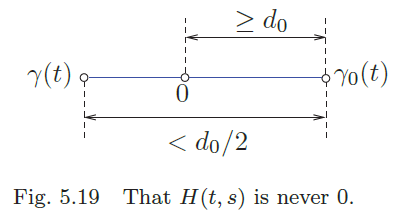
\includegraphics[width=0.4\textwidth]{./Solution/figs/fig-5-19}
\end{center}
\caption{$H(t,s)$는 $0$이 될 수 없다.}
\label{fig-5-19}
\end{figure}
직접 계산해보면,
\begin{align*}
1\cdot \dfrac{d_0}2 &> s|\gamma_0(t) - \gamma(t)|
= | \gamma_0(t) - 
\underbrace{((1-s)\gamma_0(t) + s\gamma(t))}_{=0\text{인 $t,s$를 선택할 수 있다면}}
| = |\gamma_0(t) - 0| \\
&= |\gamma_0(t)| \ge d_0.
\end{align*}
그러면, 코시 적분정리에 의해
\[
w(\gamma) = \dfrac1{2\pi i} \int_\gamma \dfrac1z dz 
= \int_{\gamma_0} \dfrac1z dz  = w(\gamma_0).
\]
\end{itemize}

\subsection*{연습문제 \ref{ex-3-22}}

\begin{figure*}[h!]
\begin{center}
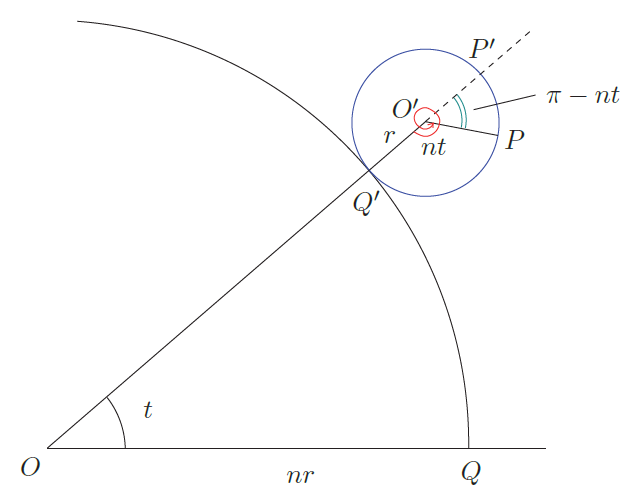
\includegraphics[width=0.4\textwidth]{./Solution/figs/fig-s-0-10}
\end{center}
%\caption{적분경로 $C$, $\tilde C$}
%\label{fig-5-18}
\end{figure*}

\begin{itemize}
\item[(1)] 큰 원의 각 $\angle Q'OQ$에 대응하는 호의 길이는 $t\cdot nr$이다.
작은 동전이 미끄러지지 않고 돌아갈 때, $O'P$와 $OO'$이 이루는 각은
$(t\cdot nr)/r = n\cdot t$이다. 그림에서 $O' \equiv (nr+r)\exp(it)$이고
\begin{align*}
P & \equiv (nr+r)\exp(it) + 
\underbrace{\exp(-i(\pi-nt))}_{\text{시계방향으로 회전}}\cdot
\underbrace{r\exp(it)}_{O'P'} \\
&=(n+1)r\exp(it) + (-1)\cdot r\cdot \exp((n+1)it).
\end{align*}
\item[(2)] 에피사이클로이드 곡선 $\gamma$로 둘러싸인 영역의 면적은
 \begin{align*}
\dfrac1{2i} \int_\gamma \bar z dz 
&= \dfrac1{2i}\int_0^{2\pi} \overline{r\left( (n+1)\exp(it)-\exp((n+1)it)\right)}\cdot \\
&\qquad\qquad r\left((n+1)i\exp(it) - (n+1)i\exp((n+1)it)\right)dt \\
&= \dfrac1{2i} \int_0^{2\pi} r^2\left( (n+1)\exp(-it) - \exp(-(n+1)it)\right)\cdot  \\
&\qquad\qquad (n+1)i\left(\exp(it) - \exp((n+1)it)\right)dt \\
&= \dfrac{(n+1)r^2}2 \int_0^{2\pi} ((n+1) -(n+1)\exp(int) - \exp(-int) +1)dt \\
&= \dfrac{(n+1)r^2}2 ((n+1) \cdot 2\pi + 0+0 + 2\pi) \\
&= (n+1)r^2\pi(n+2) = \pi r^2 (n+1)(n+2).
\end{align*}
\end{itemize}

\subsection*{연습문제 \ref{ex-3-23}}

$z\in D:= \mathbb C\setminus\{0\}$에 대하여 $f(z) = 1/z$로 정의하자.
그러면, $f$는 $D$에서 부정적분(원시함수)을 가질 수 없다.
(예제 \ref{example-3-7}\과 연습문제 \ref{ex-3-16 }\을 참고하라.)

\subsection*{연습문제 \ref{ex-3-24}}

$\gamma(t) = \exp(it)$, $t\in[0,1]$이라 하면,
\begin{align*}
\int_\gamma \dfrac i{(z-a)(az-1)}dz 
&= \int_0^{2\pi} \dfrac{i}{(\exp(it) -a)(a\exp(it)-1)}i\exp(it)dt \\
&= \int_0^{2\pi} \dfrac{-\exp(it)}{(\exp(it) -a)(a-\exp(-it))\exp(it)}dt \\
&= \int_0^{2\pi} \dfrac{1}{(\exp(it) -a)(\exp(-it)-a)}dt \\
&= \int_0^{2\pi} \dfrac1{|\exp(it)-a|^2}dt \\
&= \int_0^{2\pi} \dfrac1{((\cos t)-a)^2 + (\sin t)^2}dt \\
&= \int_0^{2\pi} \dfrac1{1-2a\cos t + a^2}dt.
\end{align*}
$0<a<1$일 때,
함수 $z\mapsto i/(ax-1)$이 단위원 $\gamma$를 포함하는 원판에서 복소해석함수이므로,
코시 적분공식에 의해
\[
\dfrac1{2\pi i} \int_\gamma \dfrac{\frac{i}{az-1}}{z-a}dz = \dfrac{i}{az-1}\Big|_{z=a}
= \dfrac i{a^2-1}.
\]
따라서,
$\dint_0^{2\pi} \dfrac 1{1-2a\cos t +a^2}dt
= \dint_\gamma \dfrac{\frac{i}{az-1}}{z-a}dz 
= 2\pi i \cdot \dfrac i{a^2-1} = \dfrac{2\pi}{1-a^2}$.

\subsection*{연습문제 \ref{ex-3-25}}

\begin{figure*}[h!]
\begin{center}
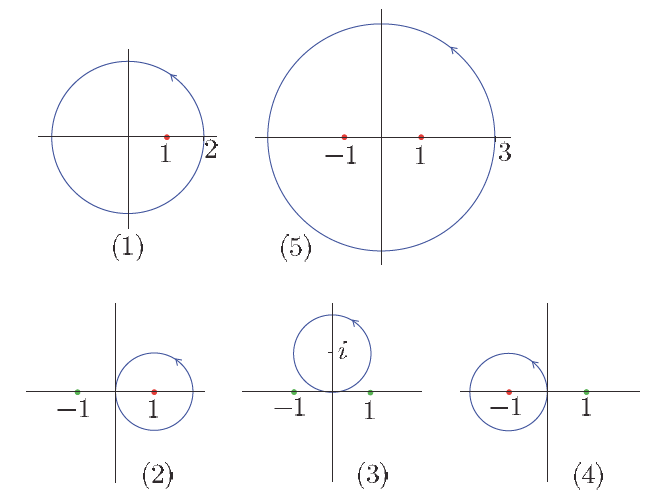
\includegraphics[width=0.7\textwidth]{./Solution/figs/fig-s-0-11}
\end{center}
%\caption{적분경로 $C$, $\tilde C$}
%\label{fig-5-18}
\end{figure*}

\begin{itemize}
\item[(1)] $\dint_\gamma \dfrac{\exp z}{z-1}dz = 2\pi i \exp z \Big|_{z=1}
= 2\pi i \exp 1 = 2\pi i  e$.
\item[(2)] $\dint_\gamma \dfrac{z^2+1}{z^2-1}dz 
= \dint_\gamma \dfrac {\frac{z^2+1}{z+1}}{z-1}dz
= 2\pi i \dfrac{z^2+1}{z+1} \Big|_{z=1} = 2\pi i \dfrac{1^2+1}{1+1} = 2\pi i$.
\item[(3)] $\dint_\gamma \dfrac{z^2+1}{z^2-1}dz = 0$.
\item[(4)] $\dint_\gamma \dfrac{z^2+1}{z^2-1}dz 
= \dint_\gamma \dfrac{\frac{z^2+1}{z-1}}{z-(-1)}dz 
= 2\pi i \dfrac{z^2+1}{z-1} \Big|_{z=-1} = 2\pi i \dfrac{(-1)^2+1}{-1-1} = -2\pi i$.
\item[(5)] $\dint_\gamma \dfrac{z^2+1}{z^2-1}dz 
= \dint_\gamma \dfrac{z^2+1}2 \left(\dfrac1{z-1} - \dfrac1{z+1}\right)dz$
\begin{align*}
\quad &= \int_\gamma \dfrac{\frac{z^2+1}2}{z-1}dz 
- \int_\gamma \dfrac{\frac{z^2+1}2}{z-(-1)}dz 
= 2\pi i \dfrac{z^2+1}2\Big|_{z=1} - 2\pi i \dfrac{z^2+1}2 \Big|_{z=-1} \\
&= 2\pi i(1) - 2\pi i (1) = 0.
\end{align*}
\end{itemize}

\subsection*{연습문제 \ref{ex-3-26}}

$F$가 부정적분이라고 하자.
원 $|z-0| = \frac12$을 반시계방향으로 도는 닫힌경로 $\gamma$를 생각하자.
경로적분의 기본정리에 의해,
\[
\dint_\gamma \dfrac1{z(z^2-1)}dz = \int_\gamma F'(z)dz = 0.
\]
한편,  코시 적분공식을 쓰면,
\[
\int_\gamma \dfrac1{z(z^2-1)}dz = \int_\gamma  \dfrac{\frac1{z^2-1}}{z-0}dz
= 2\pi i \dfrac1{z^2-1}\Big|_{z=0} = 2\pi i \dfrac1{0^2-1} = - 2\pi i.
\]
따라서 모순에 도달하게 되어
\[
\dfrac1{z(z^2-1)}
\]
은 $\{z\in\mathbb C\,:\, 0<|z|<1\}$에서 부정적분을 가질 수 없다.

\subsection*{연습문제 \ref{ex-3-27}}

\begin{figure}[h!]
\begin{center}
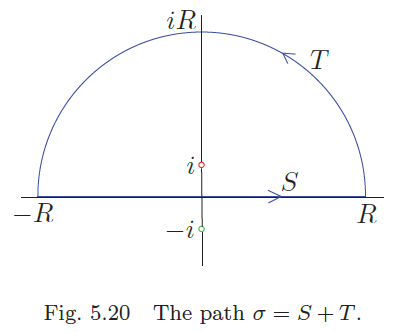
\includegraphics[width=0.4\textwidth]{./Solution/figs/fig-5-20}
\end{center}
\caption{경로 $\sigma=S+T$}
\label{fig-5-20}
\end{figure}

\begin{itemize}
\item[(1)] 코시 적분공식에 의해
\begin{align*}
\int_\sigma F(z) dz &= \int_\sigma \dfrac{\exp(iz)}{z^2+1}dz
= \int_\sigma \dfrac{\frac{\exp(iz)}{z+1}}{z-1}dz
= 2\pi i \dfrac{\exp(iz)}{z+1}\Big|_{z=i} \\
&= 2\pi i \dfrac{\exp(i\cdot i)}{i+i} = 2\pi i \dfrac{e^{-1}}{2i} = \dfrac\pi e.
\end{align*}

\item[(2)] $z=x+iy$, $x,y$는 실수이고, $y\ge0$라 하자. 그러면,
\[
|\exp(iz)| = |\exp(i(x+iy))| = |\exp(-y+ix)| = e^{-y} \le 1.
\]
따라서,
\[
|F(z)| = \dfrac{|\exp(iz)|}{|z^2+1|} \le \dfrac1{|z^2+1|}.
\]
한편, $|z^2| - |-1| \le |z^2-(-1)| = |z^2+1|$이므로,
$|z|\ge\sqrt{2}$이면,
\[
|F(z)| \le \dfrac1{|z^2+1|} \le \dfrac1{|z|^2-1} \le \dfrac2{|z|^2}.
\]
부등식을 만들 때 $|z^2|\ge 2$이면, $|z|^2\le 2|z|^2 -2$임을 이용하였다.
($|z|\ge\sqrt{2}$이면 이 조건이 만족된다)
\item[(3)] 
\begin{align*}
\left| \int_T F(z)dz \right| 
\le 2\pi R\cdot \max_{z\in T} |F(z)| &\le 2\pi R\cdot \dfrac 2{R^2} 
\quad (R\ge\sqrt{2}\text{일 때})\\
&= \dfrac{4\pi}R \stackrel{R\to\infty}{\longrightarrow} 0.
\end{align*}
따라서 $\Lim_{R\to\infty} \int_T F(z) dz = 0$.
\[
\int_S F(z)dz = \int_\sigma F(z) dz - \int_T F(z)dz = \dfrac \pi 2 -  \int_T F(z)dz
\]
이므로,  $\Lim_{R\to\infty} \int_S F(z)dz = \dfrac\pi e -\Lim_{R\to\infty} \int_T F(z)dz
= \dfrac \pi e - 0 = \dfrac \pi e$.
\item[(4)] $S(x)=x$, $x\in[-R,R]$이라 하자. 그러면,
\begin{align*}
\int_S F(z)dz &= \int_{-R}^R \dfrac{\exp(ix)}{x^2+1}\cdot 1 dx
=\int_{-R}^R \dfrac{\cos x}{x^2+1} dx 
+ i\int_{-R}^R \dfrac{\sin x}{x^2+1} dx \\
&= \int_{-R}^R \dfrac{\cos x}{x^2+1}dx  + 0
\end{align*}
마지막 등식은 $\dfrac{\sin x}{x^2+1}$이 기함수라는 성질을 이용하였다.
결론적으로,
\[
\Lim_{R\to\infty} \int_{-R}^R \dfrac{\cos x}{x^2+1}dx
= \Lim_{R\to\infty}\int_S F(z)dz = \dfrac \pi e.
\]
\end{itemize}

\subsection*{연습문제 \ref{ex-3-28}}

전해석함수 $\exp z$와 중심이 $0$이고 빈지름 $1$인 원형경로
$C:[0,2\pi] \to \mathbb C$가 $C(\theta) = \exp(i\theta)$, $\theta \in [0,2\pi]$로 
주어졌다고 하자.
코시  적분공식에 의하여,
\[
\dfrac1{2\pi i} \int_C \dfrac{\exp z}{z-0}dz = \exp z\Big|_{z=0} = \exp 0 = 1.
\]

한편,
\begin{align*}
\int_C \dfrac{\exp z}{z-0}dz 
&= \int_0^{2\pi} \dfrac{\exp(\exp(i\theta))}{\exp(i\theta)}\cdot i{\exp(i\theta)}d\theta
= i \int_0^{2\pi}  \exp(\exp(i\theta))d\theta \\
&=i \int_0^{2\pi}   \exp(\cos\theta +i\sin\theta)d\theta\\
&= i \int_0^{2\pi}  e^{\cos\theta} (\cos(\sin\theta) + i\sin(\sin\theta))d\theta\\
&= - i \int_0^{2\pi}   e^{\cos\theta} \sin(\sin\theta)d\theta 
+ i \int_0^{2\pi}     e^{\cos\theta} \cos(\sin\theta)d\theta.
\end{align*}
따라서,
$\dint_0^{2\pi} e^{\cos\theta} \cos(\sin\theta)d\theta = 2\pi$.

\subsection*{연습문제 \ref{ex-3-29}}

$f$가 복소해석함수이면, $f^{(n)}$도 복소해석함수이다.
따라서 복소미분 $f^{(n+1)}$이 존재한다.
또한, $f^{(n+1)}$이 복소미분가능하므로, 연속함수도 된다.
즉, $f^{(n)}$이 연속적으로 복소미분가능하다.

\subsection*{연습문제 \ref{ex-3-30}}

모든 $ z\in \mathbb C$에 대하여
$|f(z)| \ge \delta >0$이라고 하자.
특히, 모든 $z\in\mathbb C$에서 $f(z)\ne0$이므로
$1/f$는 전해석함수가 된다.
그런데 모든 $z\in\mathbb C$에 대하여
\[
\left| \dfrac1{f(z)}\right| \le \dfrac1\delta
\]
이므로 리우비유 정리에 의해 $1/f$는 상수함수가 되어,
$f$도 상수함수가 된다.

\subsection*{연습문제 \ref{ex-3-31}}

$z\in\mathbb C$에 대하여 $g(z):= f(z) - w_0$로  정의하자.
그러면, $g$는 전해석함수이고, 모든 $z\in\mathbb C$에 대하여  $|g(z)|\ge r$이다.
따라서 $g$는 원점에서 일정한 거리만큼 떨어져 있다.
연습문제 \ref{eq-3-30}에 의하여 $g$는 상수함수가 되므로,
$f = g +w_0$도 상수함수이다.

\subsection*{연습문제 \ref{ex-3-32}}

콤팩트 집합 $K:=\{ (x,y) \,:\, 0\le x\le T_1, 0\le y \le T_2\}$를 생각하자.
그러면 연속함수 $(x,y)\mapsto |f(x+iy)|$는 $K$에서 최댓값을 갖는다. 
최댓값을  $M$이라 하자. 
실수의 집합을 구간으로 나누면
\[
x,y\in\mathbb R = \bigcup_{n\in\mathbb Z} [ nT_1, (n+1)T_1)
= \bigcup_{m\in\mathbb Z} [ mT_1, (m+1)T_1)
\]
$x+iy = x_0 +nT_1 + i(y_0+mT_2)$을 만족하는 정수 $m$, $n$과
실수 $x_0\in [0,T_1)$, $y_0\in [0,T_2)$가 존재한다.
함수 $f$의 주기성으로부터 모든 $x,y\in\mathbb R$에 대하여
\[
f(x+iy) = f(x_0+nT_1 + i(y+0+mT_2)) = f(x_0+iy_0) \in f(K)
\]
이고, $|f(x_0+iy_0)| \le M$이다.
따라서 $f$는 $\mathbb C$ 전체에서 유계이고
리우비유 정리에 의해 상수함수가 된다.

\subsection*{연습문제 \ref{ex-3-33}}

\begin{itemize}
\item[(1)] $z\in\mathbb C$에서 $g(z)=\exp(z)\cdot f(z)$라고 정의하면
$g$는 전해석함수이다. $|f(z)| \le|\exp z|$이므로 모든 $z\in\mathbb C$에 대하여
\[
|g(z)| =| \exp(-z)\cdot f(z)| \le 1.
\]
리우비유 정리에 의해 $g$는 상수함수가 되고, 상수를 $c$라 하면,
$|g(z)|\le1$로부터 $|c|\le1$이고,
\[
g(z) = \exp(-z)\cdot f(z) = c
\]
이므로 모든 $z\in\mathbb C$에 대하여 $f(z)  = c\cdot \exp z$이다 ($|c|\le1$).

\item[(2)] $p$가 차수 $d\ge1$의 다항식이면,
$|z|>R$에 대하여
\[
|p(z)| \ge M|z|^d
\]
를 만족하는 $M, R>0$이 존재한다.
$z=x <  -R <0$로 선택하면,
$|z|>R$이고, $M|x|^d \le |p(z)| \le |e^x| = e^x \le 1$이다 ($x<0$이므로).
따라서 모든 $x<-R$에 대하여 $|x|^d \le 1/M$이 되어 모순이다.
이제 $p$가 상수함수가 되므로 상수를 $c_0$라 하자.
다시 $|p(z)| \le |\exp z|$로부터 $z=x<0$로 두면
임의의 $x<0$에 대하여
$|c_0| \le |e^x| = e^x$가 되어 $|c_0|=0$이다.
결론적으로 $p=c_0=0$을 얻는다.
\end{itemize}

\subsection*{연습문제 \ref{ex-3-34}}

\begin{itemize}
\item[(1)] $z\in C$에 대하여
\begin{align*}
|z-a_1| &\ge |z| - |a_1| = R - |a_1|, \\
|z-a_2| &\ge |z| - |a_2| = R - |a_2|
\end{align*}
이므로 
\begin{align*}
\left| \int_C \dfrac{f(z)}{(z-a_1)(z-a_2)} dz \right|
&\le \max_{z\in\mathbb C} \dfrac|{f(z)|}{|z-a_1| |z-a_2|} \cdot
(C\text{의 길이}) \\
&\le \dfrac{M}{(R-|a_1|)(R-|a_2|)}\cdot 2\pi R
\end{align*}
단, $M:= \max\limits_{z\in\mathbb C}|f(z)|$.

\item[(2)]  $a_1\ne a_2$이므로
\[
\dfrac1{z-a_1} - \dfrac1{z-a_2} = \dfrac{z-a_2 -(z-a_1)}{(z-a_1)(z-a_2)}
= \dfrac{a_1 -a_2}{(z-a_1)(z-a_2)}
\]
이고
\[
\dfrac1{(z-a_1)(z-a_2)} = \dfrac1{a_1 - a_2} \left(
\dfrac1{z-a_1} - \dfrac1{z-a_2} \right)
\]
이다. 따라서 $\alpha:=-\beta:= \dfrac1{a_1-a_2}$이다.

\item[(3)] 
\begin{align*}
\int_C \dfrac{f(z)}{(z-a_1)(z-a_2)} dz
&= \int_C \dfrac1{a_1-a_2}\left(
\dfrac1{f(z)}{z-a_1} - \dfrac{f(z)}{z-a_2} \right) dz \\
&= \dfrac1{a_1-a_2} \left( \int_C \dfrac{f(z)}{z-a_1}dz - \int_C \dfrac{f(z)}{z-a_2}dz \right).
\end{align*}
중심이 $a_1$이고 반지름 $r_1>0$인 원 $C_1$을 둘레로 하는 작은 원판 $ \Delta_1$을 생각하자.
그러면 $C$와 $C_1$은 $\mathbb C \setminus \{a_1\}$-호모토픽하고
\[
g(z):= \dfrac{f(z)}{z-a_1}, \quad z\in \mathbb C\setminus \{a_1\}
\]
는 복소해석함수이다. 코시 적분정리에 의해
\[
\int_C \dfrac{f(z)}{z-a_1}dz = \int_{C_1} \dfrac{f(z)}{z-a_1}dz.
\]
한편, 코시 적분공식을 쓰면,
$\dfrac1{2\pi i} \dint_{C_1} \dfrac{f(z)}{z-a_1}dz = f(a_1)$이므로
\[
\int_C \dfrac{f(z)}{z-a_1}dz = 2\pi i f(a_1).
\]
같은 방법으로
\[
\int_C \dfrac{f(z)}{z-a_2}dz = 2\pi i f(a_2).
\]
종합하면, $\dint_C \dfrac{f(z)}{(z-a_1)(z-a_2)} dz
= \dfrac{2\pi i(f(a_1) - f(a_2))}{a_1 - a_2}$.
\item[(4)]
$f$가 유계인 전해석함수이고 $|f|$는 상계 $M$을 갖는다고 가정하자.
즉, 모든 $z\in\mathbb C$에 대하여 $|f(z)| \le M$이다.
$a_1, a_2$가 $\mathbb C$의 서로 다른  두 점이라고 하자.
중심이 $0$이고 반지름 $R>0$인 원을 반시계방향으로 도는 경로 $C$가
$a_1, a_2$를 내부에 포함하도록 잡을 수 있다.
앞의 (1), (3)의 결과를 이용하면,
\begin{align*}
|f(a_1) - f(a_2)|
&= \dfrac{|a_1 - a_2|}{2\pi} \cdot \left| \dfrac{2\pi i(f(a_1) - f(a_2))}{a_1 - a_2} \right| \\
&= \dfrac{|a_1 - a_2|}{2\pi} \cdot \left| \int_C \dfrac{f(z)}{(z-a_1)(z-a_2)}dz \right| \\
&\le \dfrac{|a_1 - a_2|}{2\pi} \cdot \dfrac{2\pi RM}{(R-|a_1|)(R-|a_2|)}.
\end{align*}
$R$은 원하는 만큼 크게 잡을 수 있으므로, 
$R\to\infty$에 따라
\[
\dfrac{2\pi RM}{(R-|a_1|)(R-|a_2|)} \to 0
\]
이므로 $|f(a_1) - f(a_2)| =0$이다.
따라서 $f(a_1) = f(a_2)$로부터 $f$는 상수함수이다.
\end{itemize}










 